\documentclass{article}
\usepackage[europeanresistors,americaninductors,americanvoltages,americancurrents,siunitx]{circuitikz}

\usepackage{pgfplots}
%\pgfplotsset{width=7cm,compat=1.13}
\usetikzlibrary{datavisualization}
\usetikzlibrary{datavisualization.formats.functions}


\begin{document}

  \begin{circuitikz}[scale=1.2]\draw
 (0,0) node[ground] {}
 to[V=$e(t)$, *-*] (0,2) to[C=4<\nano\farad>] (2,2)
 to[R, l_=.25<\kilo\ohm>, *-*] (2,0)
 (2,2) to[R=1<\kilo\ohm>] (4,2)
 to[C, l_=2<\nano\farad>, *-*] (4,0)
 (5,0) to[I, i_=$a(t)$, -*] (5,2) -- (4,2)
 (0,0) -- (5,0)
 (0,2) -- (0,3) to[L, l=2<\milli\henry>] (5,3) -- (5,2)

 {[anchor=south east] (0,2) node {1} (2,2) node {2} (4,2) node {3}}
 ;\end{circuitikz}
	
	\begin{circuitikz}[scale=1.4]\draw
 (0,0) to[C, l=10<\micro\farad>] (0,2) -- (0,3)
 to[R, l=2.2<\kilo\ohm>] (4,3) -- (4,2)
 to[L, l=12<\milli\henry>, i=$i_1$,v=b] (4,0) -- (0,0)
 (4,2) { to[D*, *-*, color=red] (2,0) }
 (0,2) to[R, l=1<\kilo\ohm>, *-] (2,2)
 to[cV, i=1,v=$\SI{.3}{\kilo\ohm} i_1$] (4,2)
 (2,0) to[I, i=1<\milli\ampere>, -*] (2,2)
 ;\end{circuitikz}
 
 \begin{circuitikz}[scale=1.2]\draw
(0,2) to[I=1<\milli\ampere>] (2,2)
to[R, l_=2<\kilo\ohm>, *-*] (0,0)
to[R, l_=2<\kilo\ohm>] (2,0)
to[V, v_=2<\volt>] (2,2)
to[spst, l=$t_0$] (4,2) -- (4,1.5)
to [generic, i=$i_1$, v=$v_1$] (4,-.5) -- (4,-1.5)
(0,2) -- (0,-1.5) to[V, v_=4<\volt>] (2,-1.5)
to [R, l=1<\kilo\ohm>] (4,-1.5);

 \begin{scope}[xshift=6.5cm, yshift=.5cm]
 \draw [->] (-2,0) -- (2.5,0) node[anchor=west] {$v_1/\SI{}\volt$};
 \draw [->] (0,-2) -- (0,2) node[anchor=west] {$i_1/\SI{}{\milli\ampere}$} ;
 \draw (-1,0) node[anchor=north] {-2} (1,0) node[anchor=south] {2}
 (0,1) node[anchor=west] {4} (0,-1) node[anchor=east] {-4}
 (2,0) node[anchor=north west] {4}
 (-1.5,0) node[anchor=south east] {-3};
 \draw [thick] (-2,-1) -- (-1,1) -- (1,-1) -- (2,0) -- (2.5,.5);
 \draw [dotted] (-1,1) -- (-1,0) (1,-1) -- (1,0)
 (-1,1) -- (0,1) (1,-1) -- (0,-1);
 \end{scope}
 \end{circuitikz}
 \\~\\
 
      \begin{circuitikz} \draw	
      (0,2) to[V_=$e(t)$] (0,0);
 		 	\draw (0,2) to[C=$C$] (4,2) 
 			to[L=$L$] (4,0) to [R=$R$] (0,0);
 			 \draw [->] (2,1.5) to [bend left=60,edge label'=$i(t)$] (2,0.5);
 			\end{circuitikz}
 			
 			
 			\begin{circuitikz} 
 			 \draw	(0,0) to 	[L=1<\henry>](2.5,0) to [L=2<\henry>](5,0)
 			 							to	[R=1<\ohm>] (5,-2.5) to (5,-2.5)--(0,-2.5);
 			 \draw	(0,0) to 	[R,l_=1<\ohm>] (0,-1.5) to [V_=$e(t)$](0,-2.5);
    	\draw	(2.5,0) to 	[C, l=1<\farad>,*-*] (2.5,-2.5)	;
    	 \draw [->] (1.25,-0.5) to [bend left=65,edge label'=$i_1(t)$] (1.25,-2);
    	 \draw [->] (3.5,-0.5) to [bend left=65,edge label=$i_2(t)$] (3.5,-2);
 		 	\end{circuitikz}\\~\\
 		 	
\begin{tikzpicture}
\begin{axis}[
axis lines=left,
scaled ticks=false,
xticklabel style={
rotate=90,
anchor=east,
/pgf/number format/precision=3,
/pgf/number format/fixed,
/pgf/number format/fixed zerofill,
},
]
% density of Normal distribution:
\newcommand\MU{0}
\newcommand\SIGMA{1e-3}
\addplot[red,domain=-3*\SIGMA:3*\SIGMA,samples=201]
{exp(-(x-\MU)^2 / 2 / \SIGMA^2)
/ (\SIGMA * sqrt(2*pi))};
\end{axis}
\end{tikzpicture}

\begin{tikzpicture}
\begin{axis}[
axis lines=left,
scaled ticks=false,
]
% density of Normal distribution:
\newcommand\SIGMA{-6.66}

\addplot[red,domain=0:9,samples=200]
 { \SIGMA*(exp(-0.5*x)-exp(-2*x))};
\end{axis}
\end{tikzpicture}

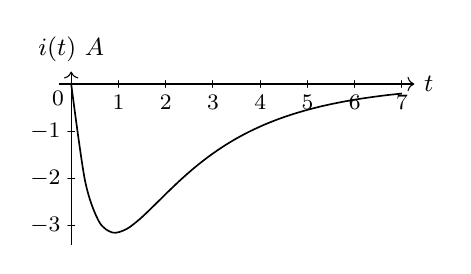
\begin{tikzpicture}[scale=0.6]
\newcommand\SIGMA{-6.66}
\datavisualization [school book axes, visualize as smooth line,x axis={label=$t$},y axis={label=$i(t)~A$}]

data [format=function] {
var x : interval [0:7];
    func y = \SIGMA*(exp(-0.5*\value x)-exp(-2*\value x));
};
\end{tikzpicture}

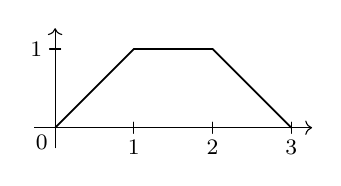
\begin{tikzpicture}
\datavisualization [school book axes, visualize as line]
data [headline={x, y}] {
0, 0
1, 1
2, 1
3, 0
};
\end{tikzpicture}

\end{document}